\newpage
	\chapter{BIODATA PENULIS 1}
	\begin{wrapfigure}{l}{0.4\textwidth}
	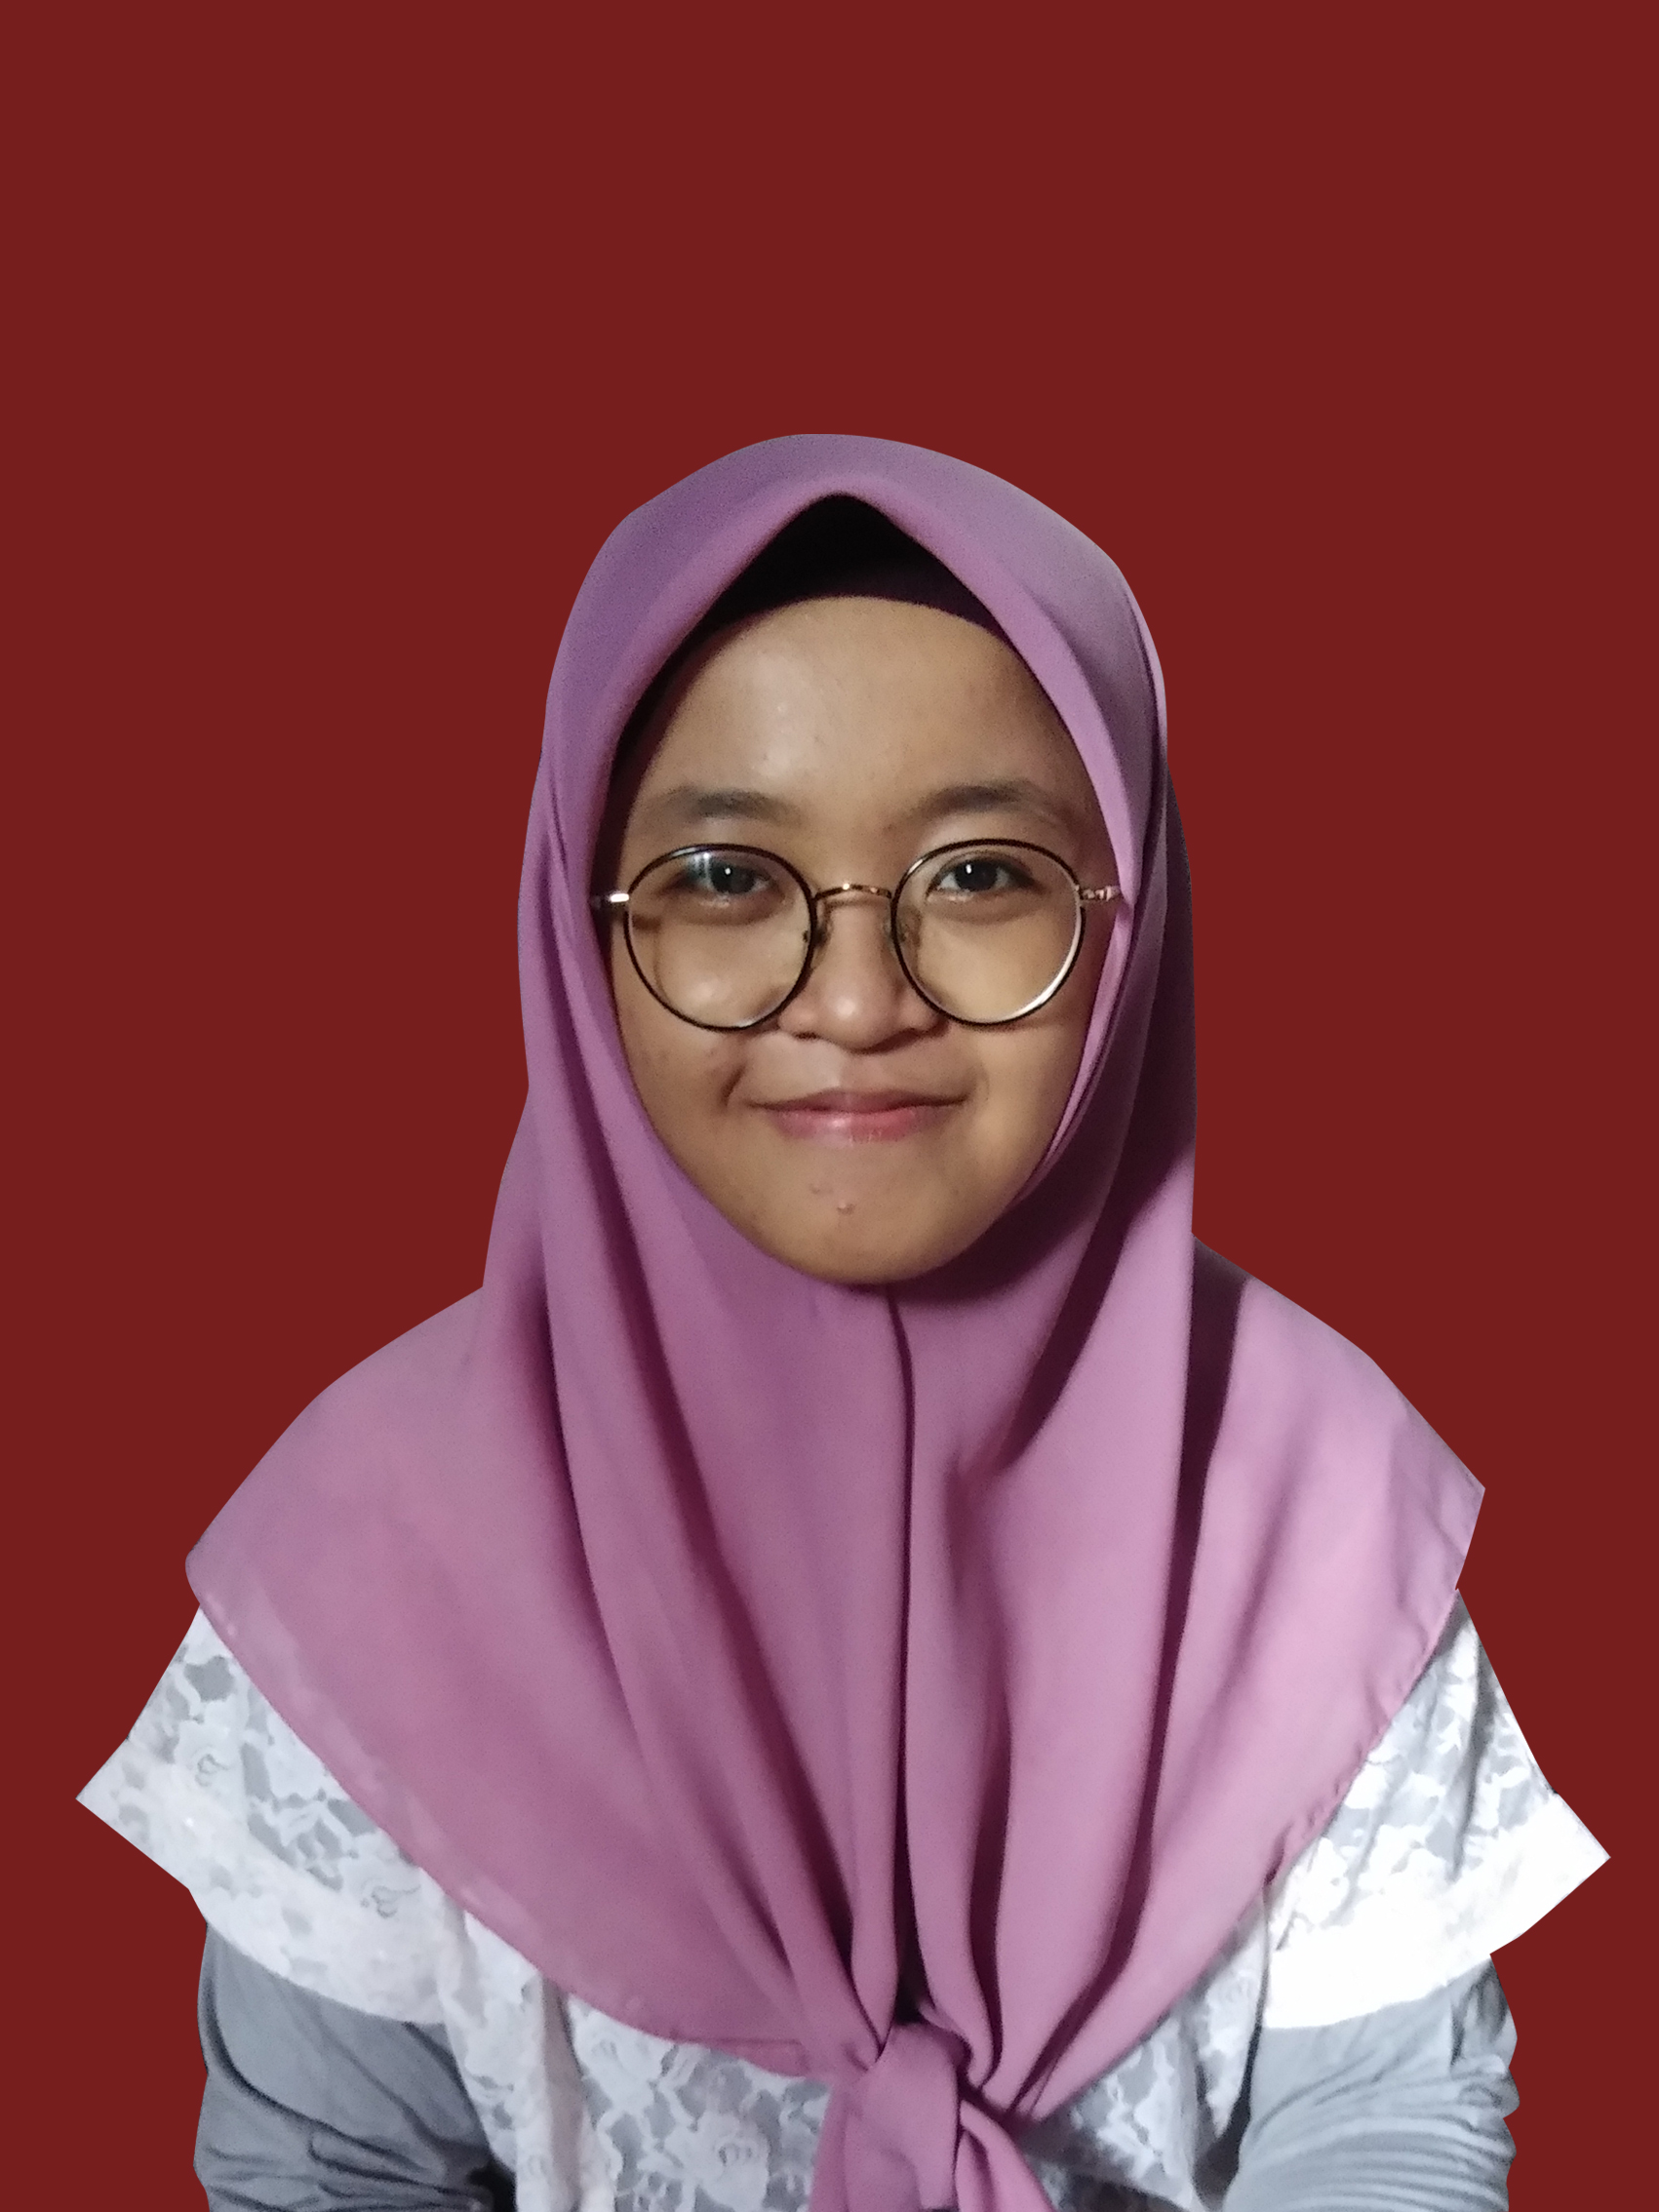
\includegraphics[height=0.3\textheight]{biodata/foto-hf.jpg}
	\end{wrapfigure}
	
	\textbf{Hafara Firdausi}, lahir di Surabaya tanggal 19 September 1998. Penulis merupakan anak pertama dari 3 bersaudara. Penulis telah menempuh pendidikan formal di TK Islam Sempoa Candi (2003-2004), SD Negeri Gelam 1 Candi (2004-2010), SMP Negeri 1 Sidoarjo (2010-2013), dan SMA Negeri 1 Sidoarjo (2013-2015). Kemudian, penulis melanjutkan studi kuliah program sarjana di Departemen Informatika, Institut Teknologi Sepuluh Nopember Surabaya. 
	
	Selama kuliah di Informatika ITS, penulis pernah menjadi asisten dosen dan praktikum untuk mata kuliah Jaringan Komputer (2017). Selama menempuh perkuliahan, penulis juga aktif di kegiatan organisasi dan kepanitiaan diantaranya menjadi staff dan staff ahli Departemen Media Informasi Himpunan Mahasiswa Teknik Computer-Informatika (HMTC) ITS, serta menjadi Badan Pengurus Harian 3D (Desain, Dekorasi, dan Dokumentasi) Schematics ITS 2017. Penulis dapat dihubungi melalui email di  \texttt{hafarafirdausi@gmail.com}.

\cleardoublepage

%nahda nnt isi sini yaa
\newpage
\chapter{BIODATA PENULIS 2}
\begin{wrapfigure}{l}{0.4\textwidth}
	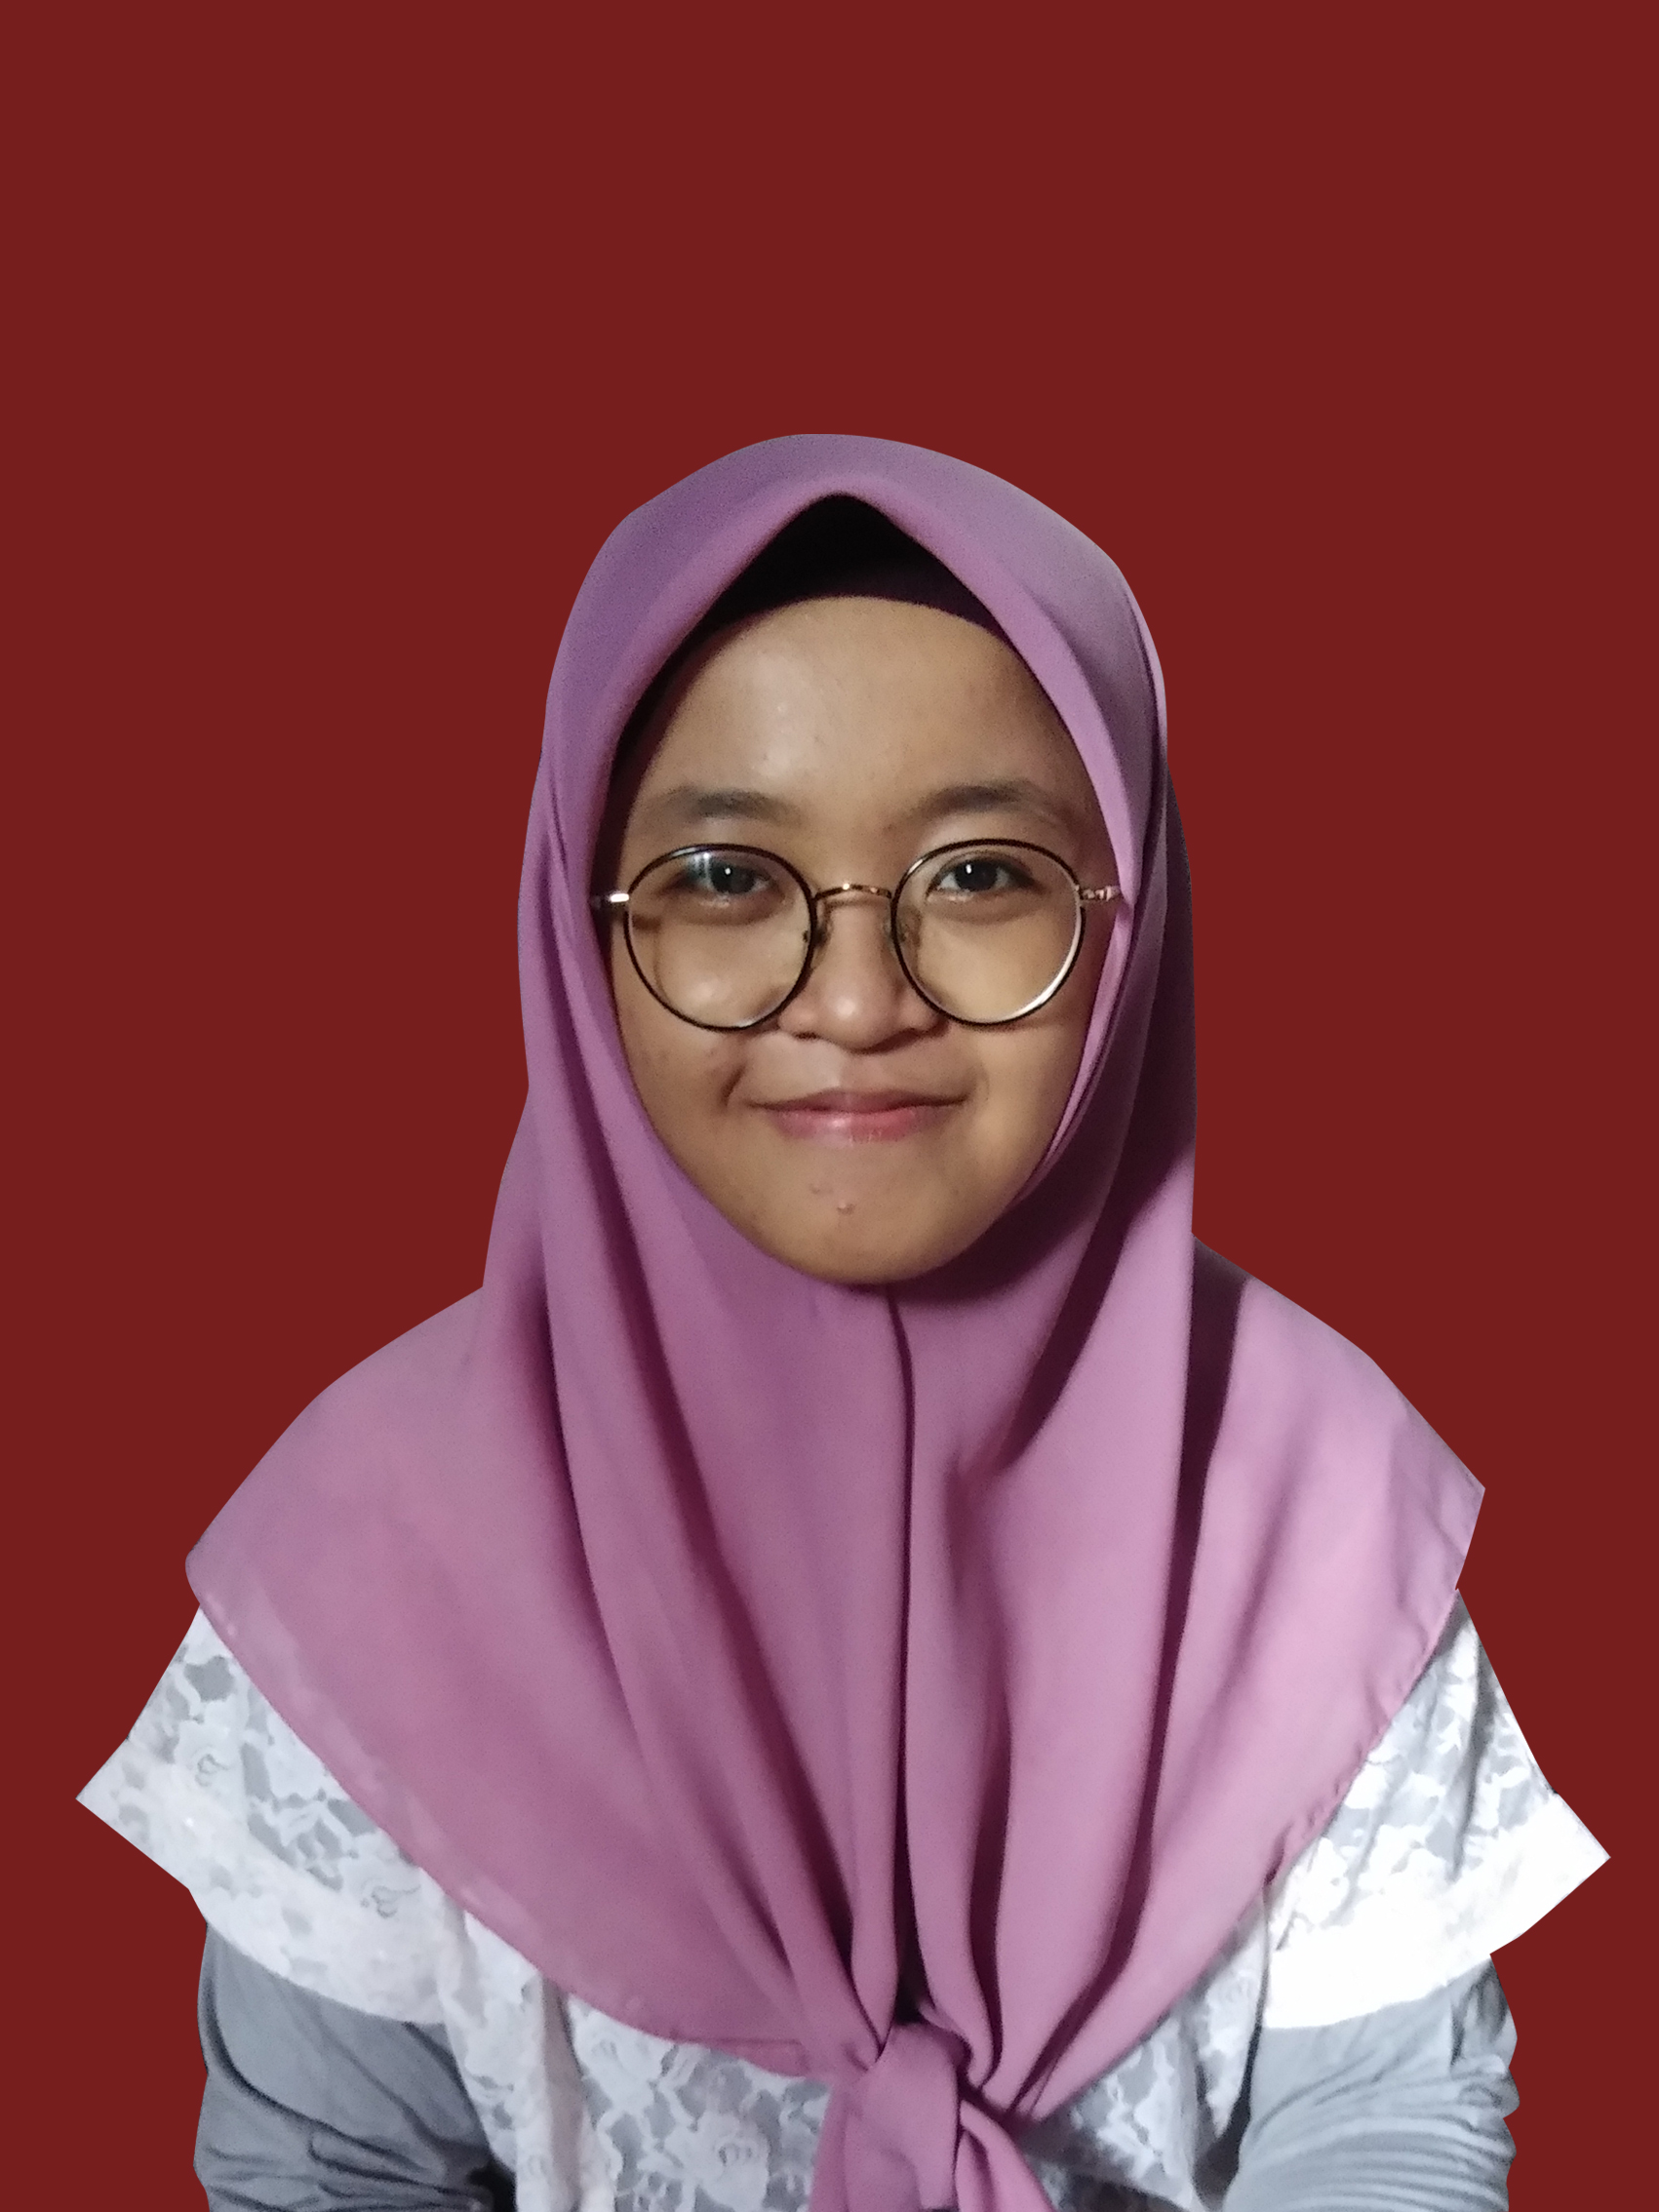
\includegraphics[height=0.3\textheight]{biodata/foto-hf.jpg}
\end{wrapfigure}

\textbf{Nahda Fauziyah Zahra}, lahir di Surabaya tanggal 19 September 1998. Penulis merupakan anak pertama dari 3 bersaudara. Penulis telah menempuh pendidikan formal di TK Islam Sempoa Candi (2003-2004), SD Negeri Gelam 1 Candi (2004-2010), SMP Negeri 1 Sidoarjo (2010-2013), dan SMA Negeri 1 Sidoarjo (2013-2015). Kemudian, penulis melanjutkan studi kuliah program sarjana di Departemen Informatika, Institut Teknologi Sepuluh Nopember Surabaya. 

Selama kuliah di Informatika ITS, penulis pernah menjadi asisten dosen dan praktikum untuk mata kuliah Jaringan Komputer (2017). Selama menempuh perkuliahan, penulis juga aktif di kegiatan organisasi dan kepanitiaan diantaranya menjadi staff dan staff ahli Departemen Media Informasi Himpunan Mahasiswa Teknik Computer-Informatika (HMTC) ITS, serta menjadi Badan Pengurus Harian 3D (Desain, Dekorasi, dan Dokumentasi) Schematics ITS 2017. Penulis dapat dihubungi melalui email di  \texttt{hafarafirdausi@gmail.com}.